%\begin{figure}[h!]
%  \centering
%  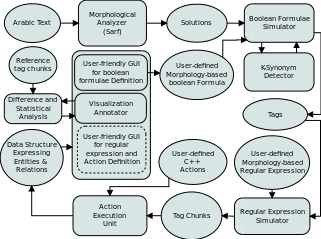
\includegraphics[width=0.45\textwidth]{figures/overview}
%  \caption{\framework Overview}
%  \label{f:overview}
%\end{figure}

\begin{figure}[h!]
\centering
\resizebox{\columnwidth}{!}
{\tiny \begin{figure}[tb!]
\centering
\resizebox{\columnwidth}{!}{
	\relsize{+1} \begin{figure}[tb!]
\centering
\resizebox{\columnwidth}{!}{
	\relsize{+1} \begin{figure}[tb!]
\centering
\resizebox{\columnwidth}{!}{
	\relsize{+1} \input{figures/overview.tex}
}
\caption{\framework flow diagram.}
\label{f:overview}
\end{figure}

Figure~\ref{f:overview} shows the flow diagram of \framework. 
%A box node represents a \framework process and 
%an ellipse node represents input and output data objects.
The Arabic text and the reference tag chunks are the primary inputs to \framework.
Solutions, morphology-based Boolean formulae, tags, 
morphology-based regular expressions, 
tag chunks, relation and action definitions, and data structures expressing entities 
and relations are input and output data to \framework processes. 
The morphological analyzer (Sarf), $Syn^k$ detector, 
GUI for Boolean formulae definition, 
visualization annotator, GUI for regular expression and action definition, 
Boolean formula simulator, regular expression simulator, 
relation extraction and action execution, and difference and statistical analyzer 
are \framework processes.

\def\pp{\ensuremath{{\cal P}}} % prefix
\def\ss{\ensuremath{{\cal S}}} % stem
\def\xx{\ensuremath{{\cal X}}} % suffix
\def\PP{\ensuremath{\mathit{POS}}} % pos
\def\GG{\ensuremath{\mathit{GLOSS}}} % gloss
\def\AC{\ensuremath{\mathit{CAT}}} % category

%~\footnote{In this document, we use the default ArabTeX transliteration style ZDMG.}
{\bf Morphological analyzer (Sarf).~}
\label{s:s:morph}
Morphological analysis is key to Arabic NLP~\cite{arabicmorph}.
Short vowels, also known as diacritics, are typically omitted in Arabic text
and inferred by readers~\cite{habash2006arabic}. 
For example, the word \RL{'sd}%
can be interpreted as \RL{'sad} {\tt ``lion''} with a {\em fatha} diacritic on the 
letter \utfrl{سـ} or 
\vocalize \RL{'sodd} (I block) with a 
{\em damma} diacritic on the letter \utfrl{سـ} and {\em shadda} on the letter \RL{d}.

In addition, the position of an Arabic letter in a word 
(beginning, middle, end, and standalone) changes
its visual form.
Some letters have non-connecting end forms which allows visual
word separation without the need of a white space separator. 
This requires morphological analysis for even the simple tokenization 
task of Arabic text.
%For example, the word \utfrl{ياسمين} can be interpreted as
%the ``Jasmine'' flower, 
%as well as \notrutfrl{يا} (the calling word) followed by
%the word \notrutfrl{سمين} (obese). 
For example, consider the sentence 
%\utfrl{ذهب الولدإلى المدرسة} 
\notrrl{AlmdrsT}\notrrl{_dhb alwald-il_A}
\arabfalse \RL{_dhb alwald-il_A almdrsT} \arabtrue
(the kid went to school). 
The letters \notrutfrl{د} and \notrutfrl{ى} have 
non-connecting end of word forms and the words 
\notrutfrl{الولد}, \notrutfrl{الى}, and  \notrutfrl{المدرسة} 
are visually separable, 
yet there is no space character in between.
Newspaper articles with text justification requirements, 
SMS messages, and automatically digitized documents
are examples where such problems often occur. 

\framework is integrated with {\em Sarf}, 
an in-house open source Arabic morphological analyzer based on 
finite state transducers~\cite{ZaMaColing2012DemosSarf}. 
Given an Arabic word, Sarf returns 
a set of morphological solutions. 
A word might have more than one solution 
due to multiple possible segmentations and multiple tags associated 
with each word. 
A morphological solution is the internal structure of the word 
composed of several morphemes including 
{\em affixes} ({\em prefixes} and {\em suffixes}), and a
{\em stem}, where each morpheme is associated with tags such as 
POS, gloss, and category tags~\cite{arabicmorph,habash2010introduction}. 
%POS, gloss,  {\em lemma}, and category tags~\cite{arabicmorph,habash2010introduction}. 
%A morpheme is the smallest linguistic unit 
%that has a meaning and fulfills a grammatical function. 

Prefixes attach before the stem and a word can have multiple prefixes. 
Suffixes attach after the stem and a word can have multiple suffixes. 
Infixes are inserted inside the stem to form a new stem. 
In this work we consider a set of stems that includes infix morphological changes. 
The part-of-speech tag, referred to as POS, 
assigns a morpho-syntactic tag for a morpheme. 
The gloss is a brief semantic notation of morpheme in English. 
A morpheme might have multiple glosses as it could stand for multiple meanings. 
The category is a user defined tag that the user can assign to several 
morphemes.
For example, the user can define a temporal category to include the 
prefix \utfrl{س} (will) and the time unit \utfrl{ساعة} (hour). 
We denote by 
\ss,
\pp,
\xx,
\PP,
\GG, and 
\AC, the set of 
all stems,
prefixes,
suffixes,
POS,
gloss, 
and user defined category tags, respectively. 

%The lemma is a convention choice that assigns a core meaning of word forms that share similar stems. 
%For example, the words \RL{byt}(house), 
%\RL{llbyt}(for the house), 
%and \RL{bywt}(houses) are mapped to the singular noun form \RL{byt} as a lemma.

\vocalize

%\setarab
\begin{table}[tb!]
  \centering
  \caption{Sample solution vector for \utfrl{فَسَيَأْكُلها}.}
  \resizebox{\columnwidth}{!}{
    \begin{tabular}{|r|c|c|c|c|c|}
          & \multicolumn{3}{c|}{\textbf{Prefixes}} & \textbf{Stem} & \textbf{Suffix} \\
    \textbf{Data} & \utfrl{فَ} & \utfrl{سَ} & \utfrl{يَ} & \utfrl{أْكُل} & \utfrl{ها} \\
    \textbf{POS} & CONJ+ & FUT+ & IV3MS+ & VERB\_IMPERFECT & IVSUFF\_DO:3FS \\
    \textbf{Gloss} & and/so & will & he/it & eat/consume & it/them/her \\
    \textbf{index} & \multicolumn{3}{c|}{10} & 13 & 16 \\
    \textbf{length} & \multicolumn{3}{c|}{3} & 3 & 2 \\
    \end{tabular}%
    }
    \vspace{-3em}
  \label{tab:samplesolution}%
\end{table}%

Table~\ref{tab:samplesolution} shows the morphological analysis
of the \utfrl{فَسَيَأْكُلها}. 
The word is composed of the prefix morphemes 
\utfrl{فَ}, \utfrl{سَ}, and \utfrl{يَ}, followed by the 
stem \utfrl{أْكُل}, and then followed by the suffix morpheme
\utfrl{ها}. 
Each morpheme is associated with a number of morphological features.
The {\tt CONJ},
{\tt FUT}, 
{\tt IV3MS} 
{\tt VERB\_IMPERFECT}, and 
{\tt IVSUFF\_DO:3FS} POS tags indicate
conjunction, 
future, 
third person masculine singular subject pronoun,
an imperfect verb, and 
and a third person feminine singular object pronoun, respectively.
The POS and gloss notations follow the Buckwalter notation~\cite{Buckwalter:02}.

%A morpheme can be a stem or an affix. 
%Each morpheme is associated with other morphological features 
%including {\em POS}, {\em gloss}, {\em lemma}, and {\em category} tags. 

%A stem can be a root word, a {\em templatic}, or {\em non-templatic} stem. 
%Templatic stems are formed from roots using template morphological rules. 
%For example, the stem
%\RL{kAtb} (writer) is a subject noun formed from the root verb \RL{ktb} (write). 
%Non-templatic stems tend to be foreign names such as \RL{واشنطن} (Washington). 
%A root is an atomic word with three, four, and rarely five letters.

%An affix can be a {\em prefix}, a {\em suffix}, or an {\em infix}. 
%The lemma is a convention choice that assigns a core meaning of word forms that share similar stems. 
%For example, the words \RL{byt}(house), 
%\RL{llbyt}(for the house), 
%and \RL{bywt}(houses) are mapped to the singular noun form \RL{byt} as a lemma.

%We introduce this feature in detail in Section~\ref{sec:framework}.

The user interacts with \framework~through a user-friendly interfaces to 
specify morphology-based Boolean formulae and regular expressions 
and associate them with tag types that are in turn associated with
visualization legends such as 
foreground and background colors and fonts. 

{\bf Boolean formula simulator.~}
\framework~uses Sarf to compute morphological solutions for the Arabic text, 
and passes the solutions along with the user-defined tag types to the 
Boolean formula simulator.
The simulator interacts with the $Syn^k$ detector, 
computes tag type matches, and produces a tag set for each word. 
%A word might have multiple tags as its morphological solutions could 
%match multiple Boolean formulae. 
%Each tag contains information about the matching word and the relevant tag type name. 
%Word information include word index relative to the text, character position, and text.
%We formally define the MBF and explain its simulation in Section~\ref{sec:framework}.

{\bf Regular expression simulator.~}
\framework~passes the sequence of tag sets and the user-defined 
tag types with morphology based regular expressions to the regular expression 
simulator. 
The simulator computes tag chunks; i.e. sequences of tags sets, that match the 
regular expressions. 
%Each tag chunk contains information about the matching sequence of words and the tag type with the matching regular expression (MRE). 
%We formally define the MRE and explain its simulation in Section~\ref{sec:framework}.

{\bf Relation extraction and action execution.~}
\framework~enables the user to associate code actions to parts of the regular
expressions. 
The user can use an API to access information such as 
text, position, length, and morphological features of the tag chunks that 
match the sub-expression. 
\framework~also allows the user to declare relations between
matches using the relation editor. 
Each relation is specified by a source, destination, and a label tuple. 
The user selects a feature of a match of sub-expressions to specify the 
tuple entities. 

\framework~executes the user-defined actions corresponding to each 
sub-expression match in a tag chunk. 
It also evaluates the semantic relation declarations against the 
tag chunks to compute the relational matches. 
Finally, \framework~uses the \cci{isA} cross-reference relation 
to create relations across tag type matches. 
%The output of this process expresses entities and relations among them. 
%We formally define the semantic relation and explain its construction in Section~\ref{sec:framework}.

{\bf Visualization annotator.~}
\framework presents the resulting tags to the user incrementally in the form of 
text annotated with style and color legends, match trees, and graphs expressing
the relational entities. 
The annotation can be edited by the user in a user-friendly interface. 
Match trees present the match text associated with the relevant tags 
and regular expression structure. 
The graphs are the result of the user defined relations.
%We present \framework's interface in Section~\ref{sec:gui}.

{\bf Agreement and statistical analysis.~}
\framework provides statistical analysis tools that help compare sets 
of tags to reference tags and compute standard agreement and accuracy measures. 
\framework~ provides criteria for comparison including exact match and intersection. 
This comparison tool can be used to edit the automatically generated annotations. 
%\framework~provides the user with an interactive interface to 
%build the reference tags. 
%We explain the analysis process and its interface in Section~\ref{sec:gui}.

}
\caption{\framework flow diagram.}
\label{f:overview}
\end{figure}

Figure~\ref{f:overview} shows the flow diagram of \framework. 
%A box node represents a \framework process and 
%an ellipse node represents input and output data objects.
The Arabic text and the reference tag chunks are the primary inputs to \framework.
Solutions, morphology-based Boolean formulae, tags, 
morphology-based regular expressions, 
tag chunks, relation and action definitions, and data structures expressing entities 
and relations are input and output data to \framework processes. 
The morphological analyzer (Sarf), $Syn^k$ detector, 
GUI for Boolean formulae definition, 
visualization annotator, GUI for regular expression and action definition, 
Boolean formula simulator, regular expression simulator, 
relation extraction and action execution, and difference and statistical analyzer 
are \framework processes.

\def\pp{\ensuremath{{\cal P}}} % prefix
\def\ss{\ensuremath{{\cal S}}} % stem
\def\xx{\ensuremath{{\cal X}}} % suffix
\def\PP{\ensuremath{\mathit{POS}}} % pos
\def\GG{\ensuremath{\mathit{GLOSS}}} % gloss
\def\AC{\ensuremath{\mathit{CAT}}} % category

%~\footnote{In this document, we use the default ArabTeX transliteration style ZDMG.}
{\bf Morphological analyzer (Sarf).~}
\label{s:s:morph}
Morphological analysis is key to Arabic NLP~\cite{arabicmorph}.
Short vowels, also known as diacritics, are typically omitted in Arabic text
and inferred by readers~\cite{habash2006arabic}. 
For example, the word \RL{'sd}%
can be interpreted as \RL{'sad} {\tt ``lion''} with a {\em fatha} diacritic on the 
letter \utfrl{سـ} or 
\vocalize \RL{'sodd} (I block) with a 
{\em damma} diacritic on the letter \utfrl{سـ} and {\em shadda} on the letter \RL{d}.

In addition, the position of an Arabic letter in a word 
(beginning, middle, end, and standalone) changes
its visual form.
Some letters have non-connecting end forms which allows visual
word separation without the need of a white space separator. 
This requires morphological analysis for even the simple tokenization 
task of Arabic text.
%For example, the word \utfrl{ياسمين} can be interpreted as
%the ``Jasmine'' flower, 
%as well as \notrutfrl{يا} (the calling word) followed by
%the word \notrutfrl{سمين} (obese). 
For example, consider the sentence 
%\utfrl{ذهب الولدإلى المدرسة} 
\notrrl{AlmdrsT}\notrrl{_dhb alwald-il_A}
\arabfalse \RL{_dhb alwald-il_A almdrsT} \arabtrue
(the kid went to school). 
The letters \notrutfrl{د} and \notrutfrl{ى} have 
non-connecting end of word forms and the words 
\notrutfrl{الولد}, \notrutfrl{الى}, and  \notrutfrl{المدرسة} 
are visually separable, 
yet there is no space character in between.
Newspaper articles with text justification requirements, 
SMS messages, and automatically digitized documents
are examples where such problems often occur. 

\framework is integrated with {\em Sarf}, 
an in-house open source Arabic morphological analyzer based on 
finite state transducers~\cite{ZaMaColing2012DemosSarf}. 
Given an Arabic word, Sarf returns 
a set of morphological solutions. 
A word might have more than one solution 
due to multiple possible segmentations and multiple tags associated 
with each word. 
A morphological solution is the internal structure of the word 
composed of several morphemes including 
{\em affixes} ({\em prefixes} and {\em suffixes}), and a
{\em stem}, where each morpheme is associated with tags such as 
POS, gloss, and category tags~\cite{arabicmorph,habash2010introduction}. 
%POS, gloss,  {\em lemma}, and category tags~\cite{arabicmorph,habash2010introduction}. 
%A morpheme is the smallest linguistic unit 
%that has a meaning and fulfills a grammatical function. 

Prefixes attach before the stem and a word can have multiple prefixes. 
Suffixes attach after the stem and a word can have multiple suffixes. 
Infixes are inserted inside the stem to form a new stem. 
In this work we consider a set of stems that includes infix morphological changes. 
The part-of-speech tag, referred to as POS, 
assigns a morpho-syntactic tag for a morpheme. 
The gloss is a brief semantic notation of morpheme in English. 
A morpheme might have multiple glosses as it could stand for multiple meanings. 
The category is a user defined tag that the user can assign to several 
morphemes.
For example, the user can define a temporal category to include the 
prefix \utfrl{س} (will) and the time unit \utfrl{ساعة} (hour). 
We denote by 
\ss,
\pp,
\xx,
\PP,
\GG, and 
\AC, the set of 
all stems,
prefixes,
suffixes,
POS,
gloss, 
and user defined category tags, respectively. 

%The lemma is a convention choice that assigns a core meaning of word forms that share similar stems. 
%For example, the words \RL{byt}(house), 
%\RL{llbyt}(for the house), 
%and \RL{bywt}(houses) are mapped to the singular noun form \RL{byt} as a lemma.

\vocalize

%\setarab
\begin{table}[tb!]
  \centering
  \caption{Sample solution vector for \utfrl{فَسَيَأْكُلها}.}
  \resizebox{\columnwidth}{!}{
    \begin{tabular}{|r|c|c|c|c|c|}
          & \multicolumn{3}{c|}{\textbf{Prefixes}} & \textbf{Stem} & \textbf{Suffix} \\
    \textbf{Data} & \utfrl{فَ} & \utfrl{سَ} & \utfrl{يَ} & \utfrl{أْكُل} & \utfrl{ها} \\
    \textbf{POS} & CONJ+ & FUT+ & IV3MS+ & VERB\_IMPERFECT & IVSUFF\_DO:3FS \\
    \textbf{Gloss} & and/so & will & he/it & eat/consume & it/them/her \\
    \textbf{index} & \multicolumn{3}{c|}{10} & 13 & 16 \\
    \textbf{length} & \multicolumn{3}{c|}{3} & 3 & 2 \\
    \end{tabular}%
    }
    \vspace{-3em}
  \label{tab:samplesolution}%
\end{table}%

Table~\ref{tab:samplesolution} shows the morphological analysis
of the \utfrl{فَسَيَأْكُلها}. 
The word is composed of the prefix morphemes 
\utfrl{فَ}, \utfrl{سَ}, and \utfrl{يَ}, followed by the 
stem \utfrl{أْكُل}, and then followed by the suffix morpheme
\utfrl{ها}. 
Each morpheme is associated with a number of morphological features.
The {\tt CONJ},
{\tt FUT}, 
{\tt IV3MS} 
{\tt VERB\_IMPERFECT}, and 
{\tt IVSUFF\_DO:3FS} POS tags indicate
conjunction, 
future, 
third person masculine singular subject pronoun,
an imperfect verb, and 
and a third person feminine singular object pronoun, respectively.
The POS and gloss notations follow the Buckwalter notation~\cite{Buckwalter:02}.

%A morpheme can be a stem or an affix. 
%Each morpheme is associated with other morphological features 
%including {\em POS}, {\em gloss}, {\em lemma}, and {\em category} tags. 

%A stem can be a root word, a {\em templatic}, or {\em non-templatic} stem. 
%Templatic stems are formed from roots using template morphological rules. 
%For example, the stem
%\RL{kAtb} (writer) is a subject noun formed from the root verb \RL{ktb} (write). 
%Non-templatic stems tend to be foreign names such as \RL{واشنطن} (Washington). 
%A root is an atomic word with three, four, and rarely five letters.

%An affix can be a {\em prefix}, a {\em suffix}, or an {\em infix}. 
%The lemma is a convention choice that assigns a core meaning of word forms that share similar stems. 
%For example, the words \RL{byt}(house), 
%\RL{llbyt}(for the house), 
%and \RL{bywt}(houses) are mapped to the singular noun form \RL{byt} as a lemma.

%We introduce this feature in detail in Section~\ref{sec:framework}.

The user interacts with \framework~through a user-friendly interfaces to 
specify morphology-based Boolean formulae and regular expressions 
and associate them with tag types that are in turn associated with
visualization legends such as 
foreground and background colors and fonts. 

{\bf Boolean formula simulator.~}
\framework~uses Sarf to compute morphological solutions for the Arabic text, 
and passes the solutions along with the user-defined tag types to the 
Boolean formula simulator.
The simulator interacts with the $Syn^k$ detector, 
computes tag type matches, and produces a tag set for each word. 
%A word might have multiple tags as its morphological solutions could 
%match multiple Boolean formulae. 
%Each tag contains information about the matching word and the relevant tag type name. 
%Word information include word index relative to the text, character position, and text.
%We formally define the MBF and explain its simulation in Section~\ref{sec:framework}.

{\bf Regular expression simulator.~}
\framework~passes the sequence of tag sets and the user-defined 
tag types with morphology based regular expressions to the regular expression 
simulator. 
The simulator computes tag chunks; i.e. sequences of tags sets, that match the 
regular expressions. 
%Each tag chunk contains information about the matching sequence of words and the tag type with the matching regular expression (MRE). 
%We formally define the MRE and explain its simulation in Section~\ref{sec:framework}.

{\bf Relation extraction and action execution.~}
\framework~enables the user to associate code actions to parts of the regular
expressions. 
The user can use an API to access information such as 
text, position, length, and morphological features of the tag chunks that 
match the sub-expression. 
\framework~also allows the user to declare relations between
matches using the relation editor. 
Each relation is specified by a source, destination, and a label tuple. 
The user selects a feature of a match of sub-expressions to specify the 
tuple entities. 

\framework~executes the user-defined actions corresponding to each 
sub-expression match in a tag chunk. 
It also evaluates the semantic relation declarations against the 
tag chunks to compute the relational matches. 
Finally, \framework~uses the \cci{isA} cross-reference relation 
to create relations across tag type matches. 
%The output of this process expresses entities and relations among them. 
%We formally define the semantic relation and explain its construction in Section~\ref{sec:framework}.

{\bf Visualization annotator.~}
\framework presents the resulting tags to the user incrementally in the form of 
text annotated with style and color legends, match trees, and graphs expressing
the relational entities. 
The annotation can be edited by the user in a user-friendly interface. 
Match trees present the match text associated with the relevant tags 
and regular expression structure. 
The graphs are the result of the user defined relations.
%We present \framework's interface in Section~\ref{sec:gui}.

{\bf Agreement and statistical analysis.~}
\framework provides statistical analysis tools that help compare sets 
of tags to reference tags and compute standard agreement and accuracy measures. 
\framework~ provides criteria for comparison including exact match and intersection. 
This comparison tool can be used to edit the automatically generated annotations. 
%\framework~provides the user with an interactive interface to 
%build the reference tags. 
%We explain the analysis process and its interface in Section~\ref{sec:gui}.

}
\caption{\framework flow diagram.}
\label{f:overview}
\end{figure}

Figure~\ref{f:overview} shows the flow diagram of \framework. 
%A box node represents a \framework process and 
%an ellipse node represents input and output data objects.
The Arabic text and the reference tag chunks are the primary inputs to \framework.
Solutions, morphology-based Boolean formulae, tags, 
morphology-based regular expressions, 
tag chunks, relation and action definitions, and data structures expressing entities 
and relations are input and output data to \framework processes. 
The morphological analyzer (Sarf), $Syn^k$ detector, 
GUI for Boolean formulae definition, 
visualization annotator, GUI for regular expression and action definition, 
Boolean formula simulator, regular expression simulator, 
relation extraction and action execution, and difference and statistical analyzer 
are \framework processes.

\def\pp{\ensuremath{{\cal P}}} % prefix
\def\ss{\ensuremath{{\cal S}}} % stem
\def\xx{\ensuremath{{\cal X}}} % suffix
\def\PP{\ensuremath{\mathit{POS}}} % pos
\def\GG{\ensuremath{\mathit{GLOSS}}} % gloss
\def\AC{\ensuremath{\mathit{CAT}}} % category

%~\footnote{In this document, we use the default ArabTeX transliteration style ZDMG.}
{\bf Morphological analyzer (Sarf).~}
\label{s:s:morph}
Morphological analysis is key to Arabic NLP~\cite{arabicmorph}.
Short vowels, also known as diacritics, are typically omitted in Arabic text
and inferred by readers~\cite{habash2006arabic}. 
For example, the word \RL{'sd}%
can be interpreted as \RL{'sad} {\tt ``lion''} with a {\em fatha} diacritic on the 
letter \utfrl{سـ} or 
\vocalize \RL{'sodd} (I block) with a 
{\em damma} diacritic on the letter \utfrl{سـ} and {\em shadda} on the letter \RL{d}.

In addition, the position of an Arabic letter in a word 
(beginning, middle, end, and standalone) changes
its visual form.
Some letters have non-connecting end forms which allows visual
word separation without the need of a white space separator. 
This requires morphological analysis for even the simple tokenization 
task of Arabic text.
%For example, the word \utfrl{ياسمين} can be interpreted as
%the ``Jasmine'' flower, 
%as well as \notrutfrl{يا} (the calling word) followed by
%the word \notrutfrl{سمين} (obese). 
For example, consider the sentence 
%\utfrl{ذهب الولدإلى المدرسة} 
\notrrl{AlmdrsT}\notrrl{_dhb alwald-il_A}
\arabfalse \RL{_dhb alwald-il_A almdrsT} \arabtrue
(the kid went to school). 
The letters \notrutfrl{د} and \notrutfrl{ى} have 
non-connecting end of word forms and the words 
\notrutfrl{الولد}, \notrutfrl{الى}, and  \notrutfrl{المدرسة} 
are visually separable, 
yet there is no space character in between.
Newspaper articles with text justification requirements, 
SMS messages, and automatically digitized documents
are examples where such problems often occur. 

\framework is integrated with {\em Sarf}, 
an in-house open source Arabic morphological analyzer based on 
finite state transducers~\cite{ZaMaColing2012DemosSarf}. 
Given an Arabic word, Sarf returns 
a set of morphological solutions. 
A word might have more than one solution 
due to multiple possible segmentations and multiple tags associated 
with each word. 
A morphological solution is the internal structure of the word 
composed of several morphemes including 
{\em affixes} ({\em prefixes} and {\em suffixes}), and a
{\em stem}, where each morpheme is associated with tags such as 
POS, gloss, and category tags~\cite{arabicmorph,habash2010introduction}. 
%POS, gloss,  {\em lemma}, and category tags~\cite{arabicmorph,habash2010introduction}. 
%A morpheme is the smallest linguistic unit 
%that has a meaning and fulfills a grammatical function. 

Prefixes attach before the stem and a word can have multiple prefixes. 
Suffixes attach after the stem and a word can have multiple suffixes. 
Infixes are inserted inside the stem to form a new stem. 
In this work we consider a set of stems that includes infix morphological changes. 
The part-of-speech tag, referred to as POS, 
assigns a morpho-syntactic tag for a morpheme. 
The gloss is a brief semantic notation of morpheme in English. 
A morpheme might have multiple glosses as it could stand for multiple meanings. 
The category is a user defined tag that the user can assign to several 
morphemes.
For example, the user can define a temporal category to include the 
prefix \utfrl{س} (will) and the time unit \utfrl{ساعة} (hour). 
We denote by 
\ss,
\pp,
\xx,
\PP,
\GG, and 
\AC, the set of 
all stems,
prefixes,
suffixes,
POS,
gloss, 
and user defined category tags, respectively. 

%The lemma is a convention choice that assigns a core meaning of word forms that share similar stems. 
%For example, the words \RL{byt}(house), 
%\RL{llbyt}(for the house), 
%and \RL{bywt}(houses) are mapped to the singular noun form \RL{byt} as a lemma.

\vocalize

%\setarab
\begin{table}[tb!]
  \centering
  \caption{Sample solution vector for \utfrl{فَسَيَأْكُلها}.}
  \resizebox{\columnwidth}{!}{
    \begin{tabular}{|r|c|c|c|c|c|}
          & \multicolumn{3}{c|}{\textbf{Prefixes}} & \textbf{Stem} & \textbf{Suffix} \\
    \textbf{Data} & \utfrl{فَ} & \utfrl{سَ} & \utfrl{يَ} & \utfrl{أْكُل} & \utfrl{ها} \\
    \textbf{POS} & CONJ+ & FUT+ & IV3MS+ & VERB\_IMPERFECT & IVSUFF\_DO:3FS \\
    \textbf{Gloss} & and/so & will & he/it & eat/consume & it/them/her \\
    \textbf{index} & \multicolumn{3}{c|}{10} & 13 & 16 \\
    \textbf{length} & \multicolumn{3}{c|}{3} & 3 & 2 \\
    \end{tabular}%
    }
    \vspace{-3em}
  \label{tab:samplesolution}%
\end{table}%

Table~\ref{tab:samplesolution} shows the morphological analysis
of the \utfrl{فَسَيَأْكُلها}. 
The word is composed of the prefix morphemes 
\utfrl{فَ}, \utfrl{سَ}, and \utfrl{يَ}, followed by the 
stem \utfrl{أْكُل}, and then followed by the suffix morpheme
\utfrl{ها}. 
Each morpheme is associated with a number of morphological features.
The {\tt CONJ},
{\tt FUT}, 
{\tt IV3MS} 
{\tt VERB\_IMPERFECT}, and 
{\tt IVSUFF\_DO:3FS} POS tags indicate
conjunction, 
future, 
third person masculine singular subject pronoun,
an imperfect verb, and 
and a third person feminine singular object pronoun, respectively.
The POS and gloss notations follow the Buckwalter notation~\cite{Buckwalter:02}.

%A morpheme can be a stem or an affix. 
%Each morpheme is associated with other morphological features 
%including {\em POS}, {\em gloss}, {\em lemma}, and {\em category} tags. 

%A stem can be a root word, a {\em templatic}, or {\em non-templatic} stem. 
%Templatic stems are formed from roots using template morphological rules. 
%For example, the stem
%\RL{kAtb} (writer) is a subject noun formed from the root verb \RL{ktb} (write). 
%Non-templatic stems tend to be foreign names such as \RL{واشنطن} (Washington). 
%A root is an atomic word with three, four, and rarely five letters.

%An affix can be a {\em prefix}, a {\em suffix}, or an {\em infix}. 
%The lemma is a convention choice that assigns a core meaning of word forms that share similar stems. 
%For example, the words \RL{byt}(house), 
%\RL{llbyt}(for the house), 
%and \RL{bywt}(houses) are mapped to the singular noun form \RL{byt} as a lemma.

%We introduce this feature in detail in Section~\ref{sec:framework}.

The user interacts with \framework~through a user-friendly interfaces to 
specify morphology-based Boolean formulae and regular expressions 
and associate them with tag types that are in turn associated with
visualization legends such as 
foreground and background colors and fonts. 

{\bf Boolean formula simulator.~}
\framework~uses Sarf to compute morphological solutions for the Arabic text, 
and passes the solutions along with the user-defined tag types to the 
Boolean formula simulator.
The simulator interacts with the $Syn^k$ detector, 
computes tag type matches, and produces a tag set for each word. 
%A word might have multiple tags as its morphological solutions could 
%match multiple Boolean formulae. 
%Each tag contains information about the matching word and the relevant tag type name. 
%Word information include word index relative to the text, character position, and text.
%We formally define the MBF and explain its simulation in Section~\ref{sec:framework}.

{\bf Regular expression simulator.~}
\framework~passes the sequence of tag sets and the user-defined 
tag types with morphology based regular expressions to the regular expression 
simulator. 
The simulator computes tag chunks; i.e. sequences of tags sets, that match the 
regular expressions. 
%Each tag chunk contains information about the matching sequence of words and the tag type with the matching regular expression (MRE). 
%We formally define the MRE and explain its simulation in Section~\ref{sec:framework}.

{\bf Relation extraction and action execution.~}
\framework~enables the user to associate code actions to parts of the regular
expressions. 
The user can use an API to access information such as 
text, position, length, and morphological features of the tag chunks that 
match the sub-expression. 
\framework~also allows the user to declare relations between
matches using the relation editor. 
Each relation is specified by a source, destination, and a label tuple. 
The user selects a feature of a match of sub-expressions to specify the 
tuple entities. 

\framework~executes the user-defined actions corresponding to each 
sub-expression match in a tag chunk. 
It also evaluates the semantic relation declarations against the 
tag chunks to compute the relational matches. 
Finally, \framework~uses the \cci{isA} cross-reference relation 
to create relations across tag type matches. 
%The output of this process expresses entities and relations among them. 
%We formally define the semantic relation and explain its construction in Section~\ref{sec:framework}.

{\bf Visualization annotator.~}
\framework presents the resulting tags to the user incrementally in the form of 
text annotated with style and color legends, match trees, and graphs expressing
the relational entities. 
The annotation can be edited by the user in a user-friendly interface. 
Match trees present the match text associated with the relevant tags 
and regular expression structure. 
The graphs are the result of the user defined relations.
%We present \framework's interface in Section~\ref{sec:gui}.

{\bf Agreement and statistical analysis.~}
\framework provides statistical analysis tools that help compare sets 
of tags to reference tags and compute standard agreement and accuracy measures. 
\framework~ provides criteria for comparison including exact match and intersection. 
This comparison tool can be used to edit the automatically generated annotations. 
%\framework~provides the user with an interactive interface to 
%build the reference tags. 
%We explain the analysis process and its interface in Section~\ref{sec:gui}.
}
\caption{\framework flow diagram.}
\label{f:overview}
\end{figure}

Figure~\ref{f:overview} shows the flow diagram of \framework.
\framework takes as input the Arabic text. 
The user interacts with \framework through a user-friendly interface to specify the
Morphology-based Boolean formulae, the Morphology-based regular expressions, 
the relation declarations, and the actions.
\framework analyzes the text using an inhouse Arabic morphological anaylzer~\cite{sarf} and computes morphological solutions
for each word in the Arabic text.
\framework passes the solutions to the Boolean formula simulator including the K-Synonym detector 
which computes the matches and produces a tag set for each word.
\framework then passes the sequence of tag sets to the regular expression simulator which computes 
chunks; i.e. sequences of words, whose tag sets match the expressions. 
\framework then evaluates the semantic relation declarations against the matches to compute the semantic relational entities, 
and executes the corresponding user-defined actions. 
Finally, \framework uses a cross-referrence relation such as the \cci{isA} relation to create relations across chunks and 
documents. 

\framework presents the resulting tags to the user incrementally in the form of 
text annotated with style and color legends, match trees, and graphs.
\framework also provides statistical analysis tools that help compare sets of tags to reference tags,
compute standard accuracy measures, and correct generated annotations. 
